\documentclass[a4paper]{report}
% Some basic packages
\usepackage[utf8]{inputenc}
\usepackage[T1]{fontenc}
\usepackage{textcomp}
\usepackage[english]{babel}
\usepackage{url}
\usepackage{graphicx}
\usepackage{float}
\usepackage{booktabs}
\usepackage{enumitem}

\pdfminorversion=7

% Don't indent paragraphs, leave some space between them
\usepackage{parskip}

% Hide page number when page is empty
\usepackage{emptypage}
\usepackage{subcaption}
\usepackage{multicol}
\usepackage{xcolor}

% Other font I sometimes use.
% \usepackage{cmbright}

% Math stuff
\usepackage{amsmath, amsfonts, mathtools, amsthm, amssymb}
% Fancy script capitals
\usepackage{mathrsfs}
\usepackage{cancel}
% Bold math
\usepackage{bm}
% Some shortcuts
\newcommand\N{\ensuremath{\mathbb{N}}}
\newcommand\R{\ensuremath{\mathbb{R}}}
\newcommand\Z{\ensuremath{\mathbb{Z}}}
\renewcommand\O{\ensuremath{\emptyset}}
\newcommand\Q{\ensuremath{\mathbb{Q}}}
\newcommand\C{\ensuremath{\mathbb{C}}}
\renewcommand\L{\ensuremath{\mathcal{L}}}

% Package for Petri Net drawing
\usepackage[version=0.96]{pgf}
\usepackage{tikz}
\usetikzlibrary{arrows,shapes,automata,petri}
\usepackage{tikzit}
\input{petri_nets_style.tikzstyles}

% Easily typeset systems of equations (French package)
\usepackage{systeme}

% Put x \to \infty below \lim
\let\svlim\lim\def\lim{\svlim\limits}

%Make implies and impliedby shorter
\let\implies\Rightarrow
\let\impliedby\Leftarrow
\let\iff\Leftrightarrow
\let\epsilon\varepsilon

% Add \contra symbol to denote contradiction
\usepackage{stmaryrd} % for \lightning
\newcommand\contra{\scalebox{1.5}{$\lightning$}}

% \let\phi\varphi

% Command for short corrections
% Usage: 1+1=\correct{3}{2}

\definecolor{correct}{HTML}{009900}
\newcommand\correct[2]{\ensuremath{\:}{\color{red}{#1}}\ensuremath{\to }{\color{correct}{#2}}\ensuremath{\:}}
\newcommand\green[1]{{\color{correct}{#1}}}

% horizontal rule
\newcommand\hr{
    \noindent\rule[0.5ex]{\linewidth}{0.5pt}
}

% hide parts
\newcommand\hide[1]{}

% si unitx
\usepackage{siunitx}
\sisetup{locale = FR}

% Environments
\makeatother
% For box around Definition, Theorem, \ldots
\usepackage{mdframed}
\mdfsetup{skipabove=1em,skipbelow=0em}
\theoremstyle{definition}
\newmdtheoremenv[nobreak=true]{definitie}{Definitie}
\newmdtheoremenv[nobreak=true]{eigenschap}{Eigenschap}
\newmdtheoremenv[nobreak=true]{gevolg}{Gevolg}
\newmdtheoremenv[nobreak=true]{lemma}{Lemma}
\newmdtheoremenv[nobreak=true]{propositie}{Propositie}
\newmdtheoremenv[nobreak=true]{stelling}{Stelling}
\newmdtheoremenv[nobreak=true]{wet}{Wet}
\newmdtheoremenv[nobreak=true]{postulaat}{Postulaat}
\newmdtheoremenv{conclusie}{Conclusie}
\newmdtheoremenv{toemaatje}{Toemaatje}
\newmdtheoremenv{vermoeden}{Vermoeden}
\newtheorem*{herhaling}{Herhaling}
\newtheorem*{intermezzo}{Intermezzo}
\newtheorem*{notatie}{Notatie}
\newtheorem*{observatie}{Observatie}
\newtheorem*{exe}{Exercise}
\newtheorem*{opmerking}{Opmerking}
\newtheorem*{praktisch}{Praktisch}
\newtheorem*{probleem}{Probleem}
\newtheorem*{terminologie}{Terminologie}
\newtheorem*{toepassing}{Toepassing}
\newtheorem*{uovt}{UOVT}
\newtheorem*{vb}{Voorbeeld}
\newtheorem*{vraag}{Vraag}

\newmdtheoremenv[nobreak=true]{definition}{Definition}
\newtheorem*{eg}{Example}
\newtheorem*{notation}{Notation}
\newtheorem*{previouslyseen}{As previously seen}
\newtheorem*{remark}{Remark}
\newtheorem*{note}{Note}
\newtheorem*{problem}{Problem}
\newtheorem*{observe}{Observe}
\newtheorem*{property}{Property}
\newtheorem*{intuition}{Intuition}
\newmdtheoremenv[nobreak=true]{prop}{Proposition}
\newmdtheoremenv[nobreak=true]{theorem}{Theorem}
\newmdtheoremenv[nobreak=true]{corollary}{Corollary}

% End example and intermezzo environments with a small diamond (just like proof
% environments end with a small square)
\usepackage{etoolbox}
\AtEndEnvironment{vb}{\null\hfill$\diamond$}%
\AtEndEnvironment{intermezzo}{\null\hfill$\diamond$}%
% \AtEndEnvironment{opmerking}{\null\hfill$\diamond$}%

% Fix some spacing
% http://tex.stackexchange.com/questions/22119/how-can-i-change-the-spacing-before-theorems-with-amsthm
\makeatletter
\def\thm@space@setup{%
  \thm@preskip=\parskip \thm@postskip=0pt
}


% Exercise 
% Usage:
% \exercise{5}
% \subexercise{1}
% \subexercise{2}
% \subexercise{3}
% gives
% Exercise 5
%   Exercise 5.1
%   Exercise 5.2
%   Exercise 5.3
\newcommand{\exercise}[1]{%
    \def\@exercise{#1}%
    \subsection*{Exercise #1}
}

\newcommand{\subexercise}[1]{%
    \subsubsection*{Exercise \@exercise.#1}
}


% \lecture starts a new lecture (les in dutch)
%
% Usage:
% \lecture{1}{di 12 feb 2019 16:00}{Inleiding}
%
% This adds a section heading with the number / title of the lecture and a
% margin paragraph with the date.

% I use \dateparts here to hide the year (2019). This way, I can easily parse
% the date of each lecture unambiguously while still having a human-friendly
% short format printed to the pdf.

\usepackage{xifthen}
\def\testdateparts#1{\dateparts#1\relax}
\def\dateparts#1 #2 #3 #4 #5\relax{
    \marginpar{\small\textsf{\mbox{#1 #2 #3 #5}}}
}

\def\@lecture{}%
\newcommand{\lecture}[3]{
    \ifthenelse{\isempty{#3}}{%
        \def\@lecture{Lecture #1}%
    }{%
        \def\@lecture{Lecture #1: #3}%
    }%
    \subsection*{\@lecture}
    \marginpar{\small\textsf{\mbox{#2}}}
}



% These are the fancy headers
\usepackage{fancyhdr}
\pagestyle{fancy}

% LE: left even
% RO: right odd
% CE, CO: center even, center odd
% My name for when I print my lecture notes to use for an open book exam.
% \fancyhead[LE,RO]{Gilles Castel}

\fancyhead[RO,LE]{\@lecture} % Right odd,  Left even
\fancyhead[RE,LO]{}          % Right even, Left odd

\fancyfoot[RO,LE]{\thepage}  % Right odd,  Left even
\fancyfoot[RE,LO]{}          % Right even, Left odd
\fancyfoot[C]{\leftmark}     % Center

\makeatother




% Todonotes and inline notes in fancy boxes
\usepackage{todonotes}
\usepackage{tcolorbox}

% Make boxes breakable
\tcbuselibrary{breakable}

% Verbetering is correction in Dutch
% Usage: 
% \begin{verbetering}
%     Lorem ipsum dolor sit amet, consetetur sadipscing elitr, sed diam nonumy eirmod
%     tempor invidunt ut labore et dolore magna aliquyam erat, sed diam voluptua. At
%     vero eos et accusam et justo duo dolores et ea rebum. Stet clita kasd gubergren,
%     no sea takimata sanctus est Lorem ipsum dolor sit amet.
% \end{verbetering}
\newenvironment{verbetering}{\begin{tcolorbox}[
    arc=0mm,
    colback=white,
    colframe=green!60!black,
    title=Opmerking,
    fonttitle=\sffamily,
    breakable
]}{\end{tcolorbox}}

% Noot is note in Dutch. Same as 'verbetering' but color of box is different
\newenvironment{noot}[1]{\begin{tcolorbox}[
    arc=0mm,
    colback=white,
    colframe=white!60!black,
    title=#1,
    fonttitle=\sffamily,
    breakable
]}{\end{tcolorbox}}




% Figure support as explained in my blog post.
\usepackage{import}
\usepackage{xifthen}
\usepackage{pdfpages}
\usepackage{transparent}
\newcommand{\incfig}[1]{%
    \def\svgwidth{\columnwidth}
    \import{./figures/}{#1.pdf_tex}
}

% Fix some stuff
% %http://tex.stackexchange.com/questions/76273/multiple-pdfs-with-page-group-included-in-a-single-page-warning
\pdfsuppresswarningpagegroup=1


% My name
\author{Bruno M. Pacheco}

 
\begin{document}

\title{Relatório 5}
\author{Bruno M. Pacheco\\
DAS 5142 - Sistemas Dinâmicos}
 
\maketitle
 
\exercise{E1}

\subsubsection*{a)}

Sem a saturação, o polinômio característico do sistema é \[
    1 + Ks(s+1)(s+p)
\]. Analisamos a estabilidade do sistema utilizando o método de Routh-Hurwitz. A matriz
\begin{center}
\begin{tabular}{c | c | c}
    $s^{3}$ & 1 & $p$ \\
    $s^{2}$ & $(1+p)$ & $50K$ \\
    $s$ & $\frac{(1+p)p-50K}{(1+p)}$ & 0 \\
    $1$ & $50K$ & 
\end{tabular}
\end{center}
nos indica que temos condições de estabilidade
\begin{align*}
    K&>0 \\
    K&<p(1+p) \\
\end{align*}
.

\subsubsection*{b)}

Agora, considerando a aproximação do elemento não linear do sistema por um ganho \[
    N(A) = \frac{4}{\pi A}
\], pode-se analisar a estabilidade do sistema no ponto crítico, \emph{i.e.}, no ponto de oscilação. Ou seja, queremos que, para um sinal de entrada com amplitude $A = 0,58$ e frequência $\omega = \sqrt{10}$ seja verdade que \[
1 + KN(A)G(j\omega) = 0
\]. Assim, encontra-se os valores de $p=10$ e $K\cong1$ como uma solução para a equação.

Encontrou-se, então, o modelo equivalente por variáveis de estado do sistema. Definiu-se como estados \[
\bm{x} = \begin{bmatrix} y(t) \\ \dot{y}(t) \\ \ddot{y}(t) \end{bmatrix} 
\] e, assim, o sistema pode ser formulado como \[
\begin{cases}
    \dot{x}_1(t) = x_2(t) \\
    \dot{x}_2(t) = x_3(t) \\
    \dot{x}_3(t) = -10x_2(t) -11x_3(t) + 50\phi\left( u(t) \right) 
\end{cases}
\] onde a entrada do sistema, em malha fechada, é $u(t) = K(y_r(t)-x_1(t))$.

Simulou-se o sistema no Simulink conforme o modelo da figura \ref{fig:figures-lab5_1_simulink_model-png}.

\begin{figure}[H]
    \centering
    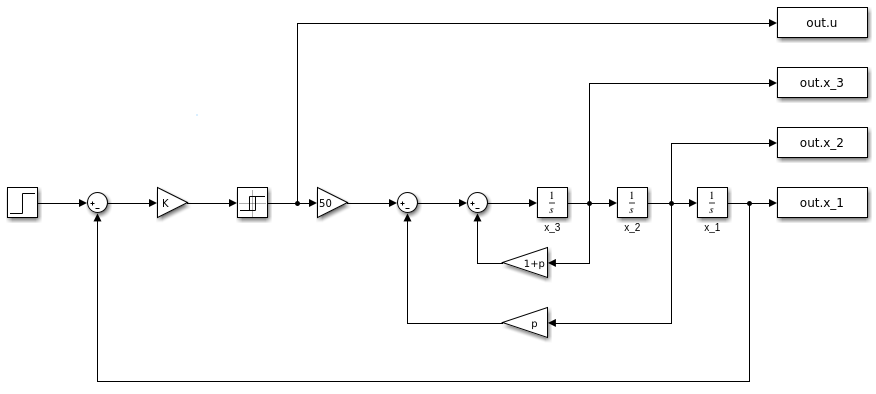
\includegraphics[width=0.8\textwidth]{figures/lab5_1_simulink_model.png}
    \caption{Modelo do sistema no \emph{Simulink}.}
    \label{fig:figures-lab5_1_simulink_model-png}
\end{figure}

Os resultados da simulação podem ser vistos nas figuras \ref{fig:figures-lab4_1_resposta_simulink}, onde podemos observar o comportamento dos estados do sistema entrando no ciclo limite e a saída, onde confirma-se a proximidade da oscilação desejada, com uma amplitude levemente maior.

\begin{figure}[H]
    \centering
    \begin{subfigure}{0.45\textwidth}
	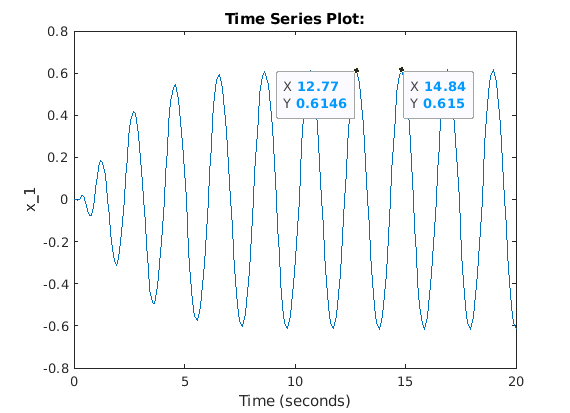
\includegraphics[width=\textwidth]{figures/lab5_1_x_1.png}
	\caption{Saída do sistema ($x_1$).}
    \end{subfigure}
    \begin{subfigure}{0.45\textwidth}
	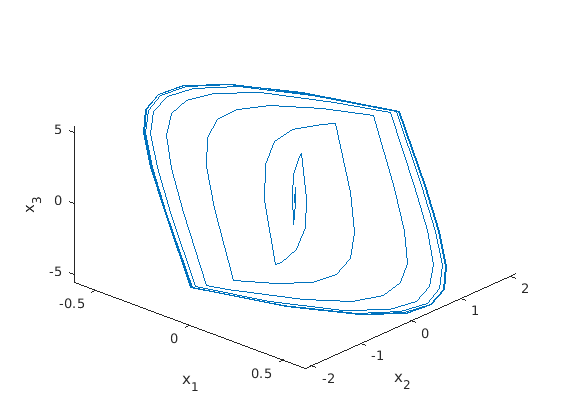
\includegraphics[width=\textwidth]{figures/lab5_1_ciclo_limite.png}
	\caption{Trajetória dos estados do sistema.}
    \end{subfigure}
    \caption{Resposta do sistema à referência nula.}
    \label{fig:figures-lab4_1_resposta_simulink}
\end{figure}

\exercise{E2}

\subsubsection*{a)}

Para o sistema idêntico ao anterior, sabemos já as características do sistema oscilando, ou seja, $A_c \cong 0,61$ e $T_{osc}\cong 2,07$. Assim, através do método de Ziegler-Nichols, projetou-se um controlador PID com parâmetros \[
\begin{cases}
    K_p = 1,25 \\
    T_i = 1,04 \\
    T_d = 0,26
\end{cases}
\].

O controlador foi realizado com uma ação \emph{anti-windup} conforme pode ser observado na figura \ref{fig:figures-lab5_2_PID-png}.

\begin{figure}[H]
    \centering
    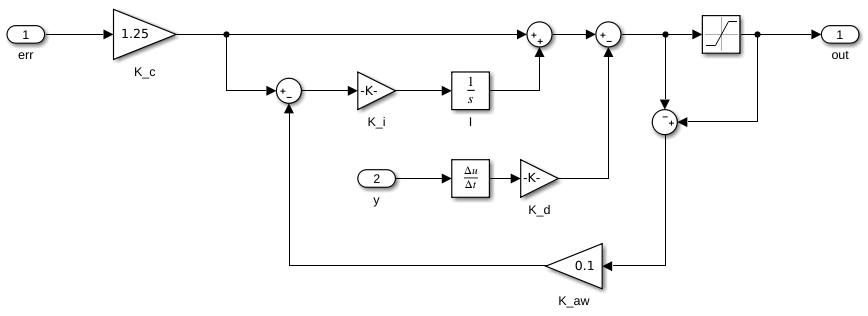
\includegraphics[width=0.8\textwidth]{figures/lab5_2_PID.png}
    \caption{Realização do controlador PID.}
    \label{fig:figures-lab5_2_PID-png}
\end{figure}

A resposta do sistema em malha fechada pode ser observada na figura \ref{fig:figures-lab5_2_a-png}. O comportamento do sistema condiz com o esperado pelo método de \emph{tuning}.

\begin{figure}[H]
    \centering
    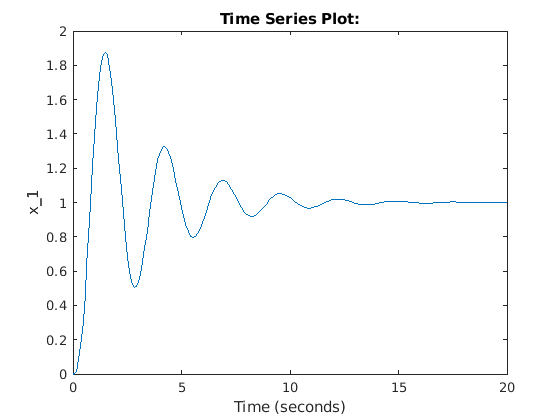
\includegraphics[width=0.8\textwidth]{figures/lab5_2_a.png}
    \caption{Resposta do sistema em malha fechada à um degrau unitário.}
    \label{fig:figures-lab5_2_a-png}
\end{figure}

\subsubsection*{b)}

Para o sistema de segunda ordem, verificou-se que a sintonia com um relé simples, sem histerese, seria impossível, uma vez que, tendo $N(A) = \frac{4M}{\pi A}$, a equação
\begin{align*}
    &G\left( j\omega \right) = \frac{-1}{N(A)} \\
    &\implies \frac{50}{-\omega^2 + 11j\omega + 10} = \frac{-\pi A}{4M} \\
    &\implies \omega^2 - 11j\omega -10 -\frac{200M}{\pi A} = 0
\end{align*}
não possui solução.

Assim, utilizou-se uma solução gráfica para definir o valor da histerese. A análise do gráfico de Nyquist de $G(j\omega)$ nos permite definir $h$ tal que a interseção entre a reta $\frac{-1}{N(A_c)}$ tenha interseção ortogonal com a trajetória de Nyquist, ou seja, para este sistema, no ponto com menor valor real. Esse valor pode ser observado na figura \ref{fig:figures-lab5_2_b_nyquist-png}.

\begin{figure}[H]
    \centering
    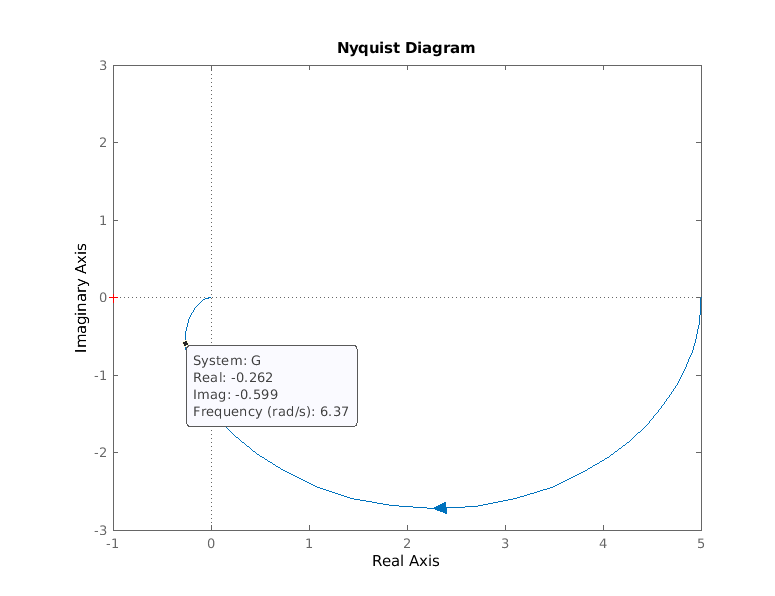
\includegraphics[width=0.8\textwidth]{figures/lab5_2_b_nyquist.png}
    \caption{Diagrama de Nyquist do segundo sistema.}
    \label{fig:figures-lab5_2_b_nyquist-png}
\end{figure}

Ou seja, adicionou-se a restrição de que a reta $\frac{-1}{N(A)}$ passe pelo ponto $-0,26 - j0,60$. Sabe-se também que
\begin{align*}
    \frac{-1}{N(A)} &= -\frac{\pi A}{4M}e^{j\sin^{-1}\left( \frac{h}{A} \right) } \\
		    &= -\frac{\pi A}{4M}\left[\sqrt{1-\left( \frac{h}{A} \right)^2 } + j\frac{h}{A}  \right] \\
.\end{align*}
Com $h<A$ para o ponto de interseção (\emph{i.e.}, assumindo que a interseção ocorre já fora da zona de histerese), temos que \[
    \Im\left\{  \frac{-1}{N(A)}\right\} = -\frac{\pi A}{4M}\frac{h}{A} = -\frac{\pi h}{4M}
\], portanto, para que a interseção se realize, utilizando um relé com $M=1$, \[
h= 0,60 \frac{4}{\pi} \cong 0,76
\].

Então, avaliando o polinômio característico na frequência de interseção $\omega_c \cong 6,37$, tem-se
\begin{align*}
    &G(j\omega) = \frac{-1}{N(A_c)} \\
    &\implies \frac{200M}{\pi A_c}\left[\sqrt{1-\left( \frac{h}{A_c} \right)^2 } -j \frac{h}{A_c} \right] = \omega_c^2 - 11j\omega_c - 10 \\
    &\alpha := \frac{h}{A_c} \implies 83,77 \alpha \left[\sqrt{1-\alpha^2 } -j \alpha \right] = \omega_c^2 - 11j\omega_c - 10 \\
\end{align*}
. Igualando as partes imaginárias, tem-se
\begin{align*}
    &\omega_c = 7,62 \alpha^2 \\
    &\implies \alpha = \sqrt{\frac{\omega_c}{7,62}} \\
    &\implies A_c \cong 0,83
.\end{align*}

Verificou-se, então, esses resultados através da simulação. O resultado pode ser observado na figura \ref{fig:figures-lab5_2_b_x_1-png}. Pode-se observar uma boa aproximação dos valores calculados, tanto para a amplitude quanto para a frequência de oscilação, validando-os.

\begin{figure}[H]
    \centering
    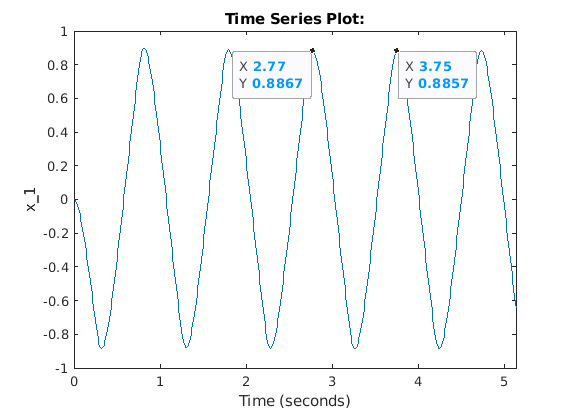
\includegraphics[width=0.6\textwidth]{figures/lab5_2_b_x_1.png}
    \caption{Saída do sistema à referência nula utilizando o relé com histerese com os parâmetros calculados}
    \label{fig:figures-lab5_2_b_x_1-png}
\end{figure}

Em seguida, projetou-se o controlador PID com parâmetros \[
\begin{cases}
    K_p = 0,92 \\
    T_i = 0,49 \\
    T_d = 0,12
\end{cases}
\] e implementou-o utilizando o mesmo arranjo apresentado previamente. Os resultados podem ser observados na figura \ref{fig:figures-lab5_2_b_resultado-png}. A resposta do sistema apresenta comportamento esperado dado o método de Ziegler-Nichols.

\begin{figure}[H]
    \centering
    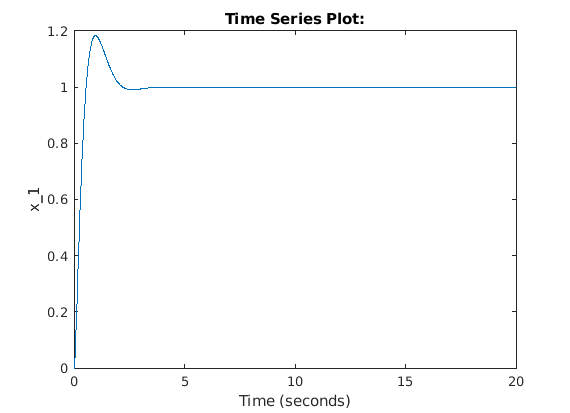
\includegraphics[width=0.6\textwidth]{figures/lab5_2_b_resultado.png}
    \caption{Resposta ao degrau unitário do sistema com o controlador projetado.}
    \label{fig:figures-lab5_2_b_resultado-png}
\end{figure}

\end{document}
